\section{Data Warehouse Design}

\subsection{Mục tiêu thiết kế}
Kho dữ liệu được xây dựng để phục vụ hai nhu cầu chính: phân tích kinh doanh bằng Power BI và lưu trữ dữ liệu khoản vay theo cấu trúc ổn định, dễ truy vấn. Luồng triển khai của phần này là:

\begin{center}
\texttt{living\_sample\_100k.csv} $\rightarrow$ \texttt{stg.Loan\_Raw} $\rightarrow$ \texttt{dw.Dim\_*} $\rightarrow$ \texttt{dw.Fact\_Loan}
\end{center}

File \texttt{living\_sample\_100k.csv} là đầu ra của bước ETL trong notebook, giữ phân phối tự nhiên của dữ liệu kinh doanh để các dashboard phản ánh đúng tỷ lệ thực tế. File này được nạp vào SQL Server bằng script \texttt{import\_to\_sql.py}, sau đó script \texttt{sql/loan\_db.sql} tạo staging schema, data warehouse schema và nạp dữ liệu vào các bảng theo mô hình sao.

\subsection{Logical Design: Star Schema}
Nhóm thiết kế Data Warehouse theo mô hình \textbf{Star Schema}. Mô hình này có một bảng fact trung tâm kết nối với các bảng dimension thông qua khóa ngoại.

\subsubsection{Grain của bảng Fact}
Grain của bảng \texttt{dw.Fact\_Loan} là:

\begin{quote}
Mỗi dòng trong \texttt{Fact\_Loan} đại diện cho một hồ sơ khoản vay hợp lệ sau khi loại bỏ trạng thái \textit{Current} và các lỗi logic tài chính.
\end{quote}

Các measure chính trong bảng fact gồm:
\begin{itemize}
    \item \texttt{loan\_amnt}: số tiền vay.
    \item \texttt{int\_rate}: lãi suất khoản vay.
    \item \texttt{installment}: khoản trả góp hàng tháng.
    \item \texttt{loan\_status\_bin}: nhãn rủi ro dùng cho phân tích, trong đó 0 là hồ sơ tốt và 1 là hồ sơ xấu/trễ hạn.
\end{itemize}

\subsubsection{Các bảng Dimension}
\begin{itemize}
    \item \textbf{\texttt{dw.Dim\_Borrower}:} mô tả đặc điểm người vay, gồm \texttt{emp\_length}, \texttt{home\_ownership}, \texttt{annual\_inc}, \texttt{income\_bin}, \texttt{dti}, \texttt{delinq\_2yrs}, \texttt{total\_acc}.
    \item \textbf{\texttt{dw.Dim\_Loan\_Info}:} mô tả đặc điểm khoản vay, gồm \texttt{term}, \texttt{grade}, \texttt{verification\_status}.
\end{itemize}

\textit{Ghi chú kỹ thuật:} \texttt{Dim\_Borrower} hiện chứa một số thuộc tính định lượng như \texttt{annual\_inc}, \texttt{dti} và \texttt{total\_acc}, nên dimension này có cardinality cao. Với phạm vi bài tập lớn, thiết kế này vẫn chấp nhận được vì giúp Power BI phân tích trực tiếp theo thông tin người vay. Để tối ưu hơn trong hệ thống sản xuất, có thể chuyển một phần biến định lượng sang bảng fact hoặc chỉ giữ các biến đã được phân thùng như \texttt{income\_bin}.

\begin{figure}[H]
    \centering
    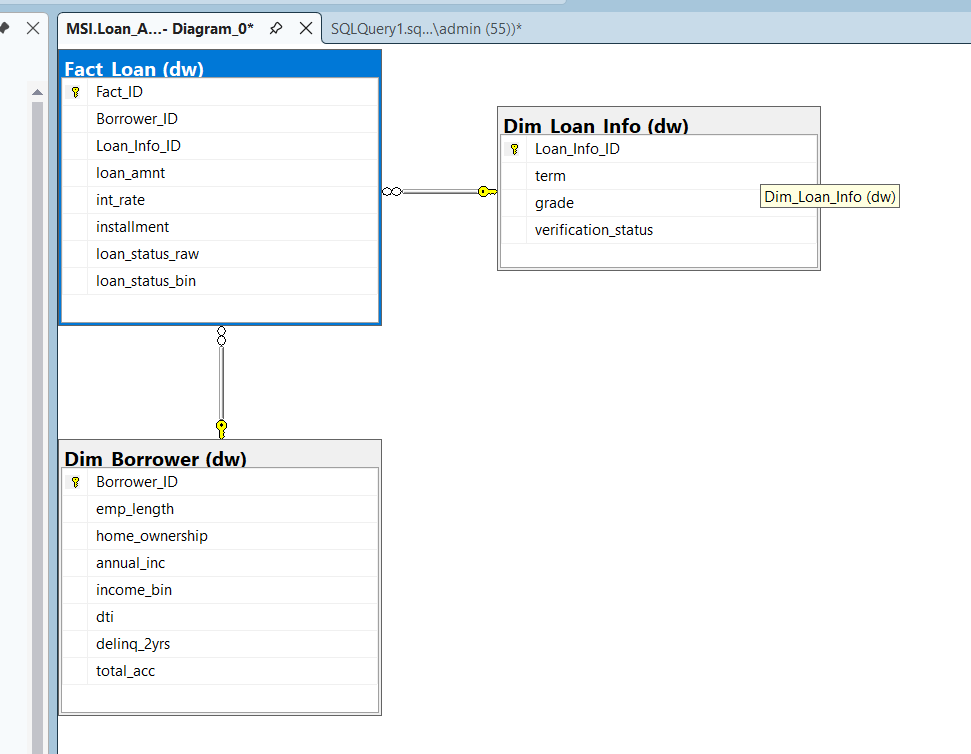
\includegraphics[width=0.8\textwidth]{images/Screenshot 2026-05-14 083154.png}
    \caption{Sơ đồ Star Schema của Data Warehouse khoản vay}
    \label{fig:star_schema}
\end{figure}

\subsection{Physical Design trên SQL Server}
Cấu trúc vật lý được chia thành hai schema:
\begin{itemize}
    \item \textbf{\texttt{stg}:} chứa bảng staging \texttt{stg.Loan\_Raw}, là nơi nhận dữ liệu từ file CSV.
    \item \textbf{\texttt{dw}:} chứa các bảng đã được tổ chức theo mô hình sao, gồm \texttt{dw.Dim\_Borrower}, \texttt{dw.Dim\_Loan\_Info} và \texttt{dw.Fact\_Loan}.
\end{itemize}

Script nạp dữ liệu \texttt{import\_to\_sql.py} ưu tiên đọc file \texttt{data/processed/living\_sample\_100k.csv}. Nếu file này chưa tồn tại, script mới dùng fallback là \texttt{data/raw/loan\_dw.csv}. Cách này đảm bảo nguồn nạp vào kho dữ liệu là output chính thức của bước ETL.

\subsection{ETL trong SQL Server}
Dựa trên file \texttt{sql/loan\_db.sql}, quá trình ETL trong SQL Server gồm ba bước:
\begin{enumerate}
    \item \textbf{Extract:} import CSV vào bảng \texttt{dbo.Loan\_Raw}, sau đó chuyển sang schema \texttt{stg}.
    \item \textbf{Transform:} lọc lỗi logic tài chính, loại trạng thái \textit{Current}, điền \texttt{Unknown} cho \texttt{emp\_length}, tạo \texttt{income\_bin} và chuyển \texttt{loan\_status} thành \texttt{loan\_status\_bin}.
    \item \textbf{Load:} nạp dữ liệu vào dimension trước, sau đó nạp fact bằng cách join với dimension để lấy surrogate key.
\end{enumerate}

\subsubsection{Business Logic trong SQL}
Các transformation quan trọng được thực hiện trực tiếp trong SQL:
\begin{itemize}
    \item \textbf{Data cleaning:} chỉ giữ hồ sơ có \texttt{annual\_inc > 0}, \texttt{dti >= 0}, \texttt{loan\_amnt > 0}, \texttt{installment > 0}; loại các dòng thiếu ở \texttt{delinq\_2yrs} và \texttt{total\_acc}.
    \item \textbf{Missing value handling:} chuyển \texttt{emp\_length} bị thiếu thành \texttt{Unknown}.
    \item \textbf{Data binning:} phân thùng \texttt{annual\_inc} thành \textit{Low Income}, \textit{Medium Income}, \textit{High Income}.
    \item \textbf{Target transformation:} chuyển \texttt{loan\_status} thành \texttt{loan\_status\_bin}. \textit{Fully Paid} và credit-policy fully paid được gán 0; \textit{Charged Off}, \textit{Default}, credit-policy charged off và các trạng thái \textit{Late} được gán 1.
\end{itemize}

\begin{lstlisting}[language=SQL, caption=Trích đoạn SQL tạo dimension và fact]
INSERT INTO dw.Dim_Borrower
    (emp_length, home_ownership, annual_inc, income_bin, dti, delinq_2yrs, total_acc)
SELECT DISTINCT
    ISNULL(CAST(emp_length AS NVARCHAR(50)), 'Unknown') AS emp_length,
    CAST(home_ownership AS NVARCHAR(50)),
    annual_inc,
    CASE
        WHEN annual_inc < 50000 THEN 'Low Income (<50k)'
        WHEN annual_inc >= 50000 AND annual_inc <= 100000 THEN 'Medium Income (50k-100k)'
        WHEN annual_inc > 100000 THEN 'High Income (>100k)'
        ELSE 'Unknown'
    END AS income_bin,
    dti, delinq_2yrs, total_acc
FROM stg.Loan_Raw
WHERE loan_status != 'Current'
  AND annual_inc > 0
  AND dti >= 0
  AND loan_amnt > 0
  AND installment > 0
  AND delinq_2yrs IS NOT NULL
  AND total_acc IS NOT NULL;

INSERT INTO dw.Fact_Loan
    (Borrower_ID, Loan_Info_ID, loan_amnt, int_rate, installment, loan_status_raw, loan_status_bin)
SELECT
    b.Borrower_ID,
    l.Loan_Info_ID,
    r.loan_amnt,
    r.int_rate,
    r.installment,
    r.loan_status,
    CASE
        WHEN r.loan_status IN ('Fully Paid',
             'Does not meet the credit policy. Status:Fully Paid') THEN 0
        WHEN r.loan_status IN ('Charged Off', 'Default',
             'Does not meet the credit policy. Status:Charged Off')
             OR r.loan_status LIKE '%Late%' THEN 1
        ELSE NULL
    END AS loan_status_bin
FROM stg.Loan_Raw r
JOIN dw.Dim_Borrower b
    ON ISNULL(CAST(r.emp_length AS NVARCHAR(50)), 'Unknown') = b.emp_length
    AND CAST(r.home_ownership AS NVARCHAR(50)) = b.home_ownership
    AND r.annual_inc = b.annual_inc
    AND r.dti = b.dti
    AND r.delinq_2yrs = b.delinq_2yrs
    AND r.total_acc = b.total_acc
JOIN dw.Dim_Loan_Info l
    ON CAST(r.term AS NVARCHAR(50)) = l.term
    AND CAST(r.grade AS NVARCHAR(50)) = l.grade
    AND CAST(r.verification_status AS NVARCHAR(50)) = l.verification_status
WHERE r.loan_status != 'Current'
  AND r.annual_inc > 0
  AND r.dti >= 0
  AND r.loan_amnt > 0
  AND r.installment > 0
  AND r.delinq_2yrs IS NOT NULL
  AND r.total_acc IS NOT NULL;
\end{lstlisting}

\subsection{Kiểm tra số dòng sau khi load}
Sau khi chạy \texttt{loan\_db.sql} trên file \texttt{living\_sample\_100k.csv}, số dòng kỳ vọng của các bảng như sau:

\begin{table}[H]
    \centering
    \renewcommand{\arraystretch}{1.2}
    \begin{tabular}{|l|r|l|}
        \hline
        \textbf{Bảng} & \textbf{Số dòng} & \textbf{Vai trò} \\ \hline
        \texttt{stg.Loan\_Raw} & 100.000 & Bảng staging nhận dữ liệu từ CSV \\ \hline
        \texttt{dw.Dim\_Borrower} & 59.314 & Dimension người vay \\ \hline
        \texttt{dw.Dim\_Loan\_Info} & 42 & Dimension thông tin khoản vay \\ \hline
        \texttt{dw.Fact\_Loan} & 59.337 & Fact khoản vay sau khi loại \textit{Current} và lỗi logic \\ \hline
    \end{tabular}
    \caption{Số dòng kỳ vọng sau khi load Data Warehouse}
    \label{tab:dwh_row_counts}
\end{table}

File SQL cũng có truy vấn kiểm tra cuối script để xác nhận số dòng thực tế sau khi load:

\begin{lstlisting}[language=SQL, caption=Truy vấn kiểm tra số dòng trong Data Warehouse]
SELECT 'stg.Loan_Raw' AS table_name, COUNT(*) AS row_count FROM stg.Loan_Raw
UNION ALL
SELECT 'dw.Dim_Borrower', COUNT(*) FROM dw.Dim_Borrower
UNION ALL
SELECT 'dw.Dim_Loan_Info', COUNT(*) FROM dw.Dim_Loan_Info
UNION ALL
SELECT 'dw.Fact_Loan', COUNT(*) FROM dw.Fact_Loan;
\end{lstlisting}

\begin{figure}[H]
    \centering
    \includegraphics[width=0.8\textwidth]{images/Screenshot 2026-05-16 135802.png} % Thay đổi tên file nếu cần
    \caption{Kết quả kiểm chứng dữ liệu sau quá trình ETL trong SQL Server}
    \label{fig:etl_results}
\end{figure}
Dựa trên Hình \ref{fig:etl_results}, kết quả thực thi các truy vấn kiểm tra cho thấy quá trình trích xuất và biến đổi dữ liệu (ETL) đã hoàn tất thành công. Cụ thể:
\begin{itemize}
    \item Tổng số dòng dữ liệu sạch được nạp vào bảng \textit{Fact\_Loan} là 59,337 dòng (đã loại bỏ các bản ghi không phù hợp).
    \item Biến mục tiêu (\textit{loan\_status\_bin}) đã được chuyển đổi chính xác sang dạng nhị phân: 0 (Nợ tốt) và 1 (Nợ xấu), sẵn sàng cho việc huấn luyện mô hình Machine Learning.
    \item Dữ liệu trong View \textit{vw\_Loan\_Dashboard} khớp hoàn toàn với bảng Fact, đảm bảo tính toàn vẹn dữ liệu cho báo cáo Power BI.
\end{itemize}
